
% Title: Container-based server consolidation using Evolutionary
% Computation methods

\section{Problem Statement}

% Cloud computing is a computing model offering a network of servers to their clients in a on-demand fashion. It provides great flexibility to application providers who can simply start their businesses by deploying their applications on Cloud servers. With elastic resource management system, Cloud provides unlimited resources to application with a pay-as-you-go policy. This fundamentally changes the software industry.

% As the virtualization technology evolves, a new trend of container-based Cloud \cite{Felter:2015ki, Dua:2014uza} emerges in recent years and quickly become a hot topic in both industry and acedemia.A corresponding service model: Container as a Service \cite{Piraghaj:2015uf} is proposed in order to overcome the disadvantages (see details in Section \ref{sec:}) of traditional service models: the over-provisioning problem in Infrastructure as a Service (IaaS) and the restricted software development environment in Platform as a Service (PaaS). Overall, container technology provides a finer granularity level of resource management than VM-based virtualization which can dramatically alleviate the over-provisioning problem. Furthermore, containers support user-defined libraries which solve the lock-in problem \cite{Armbrust:2010vq} in PaaS.

% However, the new technology also brings new challenges to resource optimization. 



% From NIST's definition \cite{Mell:2011jj}, \textit{"cloud computing is a model for enabling ubiquitous, convenient, on-demand network access to a shared pool of configurable computing resources (e.g., networks, servers, storage, applications and services) that can be rapidly provisioned and released with minimal management effort or service provider interaction."} 
To illustrate how it works, considering the case: a Cloud provider builds a data center which contains thousands of servers connected with network. These servers are virtualized which means they are partitioned into a smaller unit of resources called \emph{Virtual Machines (VMs)} or \emph{Containers}. A web-based application provider can access and deploy their applications (e.g Endnote, Google Drive and etc.) in these resource units from anywhere in the world. Once the applications start serving, application users can use them without installing on their local computers.

Cloud providers offer the fundamental resources: data centers and computation powers that support the modern Cloud computing industry, software industry and etc. Therefore, reducing the cost of data centers will lead to a reduction of cost of softwares which consequently be beneficial to most people who access the Internet on a daily basis.

In this thesis, our goal is to help Cloud providers to reduce expense from the energy consumption by servers in data centers because energy is the major source of expense \cite{Kaplan:up01fR-k}. Specifically, we achieve this goal by providing better resource allocation techniques based on container technology and server consolidation to optimize the resource utilization in three resource allocation scenarios.

The problem can be described as, given a number of Physical Machines (PMs) which can be represented as the resources such as a number of CPU cores and memory they contained; a number of different fixed configurations of VMs, each configuration can also be represented as aforementioned resources; and a number of containers which represent the resource requirements of applications. The task is to allocate these containers to a number of different VMs. Furthermore, allocating these VMs to a number of PMs. The objective is to minimize the number of PMs used to accommodate these containers. The decision variable is the location of containers and VMs as well as the selection of the configurations of VMs. The constraints are the aggregated resources of containers inside a VM cannot exceed the VM's capacity. Similarly, the aggregated resources of VMs inside a PM cannot exceed the PM's capacity. The task is generally considered as a server consolidation problem.

\begin{figure}
	\centering
	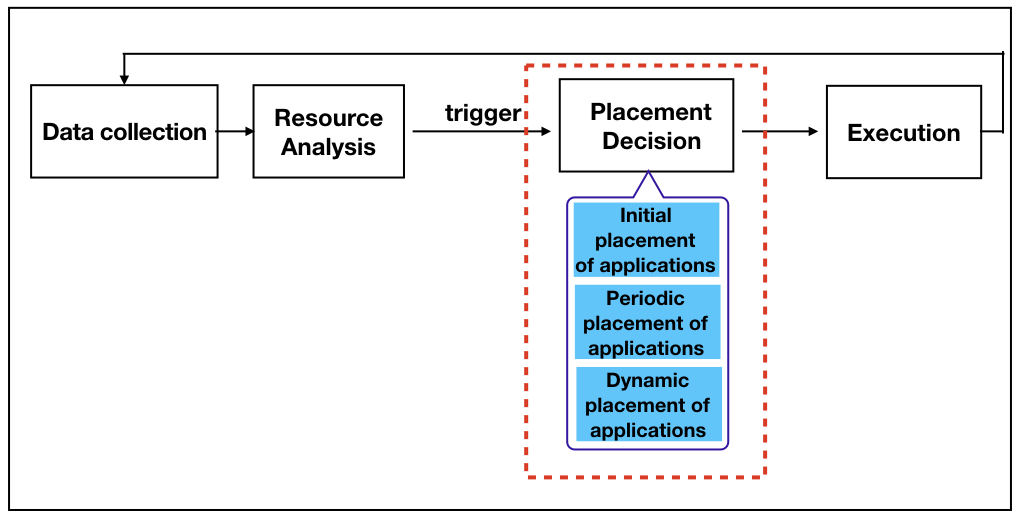
\includegraphics[width=0.7\textwidth]{pics/workflow_management.png}
	\caption{A workflow of resource management \cite{Mishra:2012kx}}
	\label{fig:workflow}
\end{figure}

Server consolidation problems have different assumptions, objectives and requirements in multiple resource re-allocation scenarios as shown in Figure \ref{fig:workflow} including new application allocation, periodic optimization, overloading and under-loading adjustment.
Periodic optimization can be seen as static server consolidation, because these optimization normally involves large amount of variables, therefore, it is quite time-consuming. It takes a number of existing applications and re-allocate them into a number of PMs. This problem is conducted in an off-line fashion. Overloading and under-loading can be categories to dynamic consolidation problem, since they consider allocating one application each time and require a fast on-line operation. New application allocation can be seen as either static: allocate a batch of new applications, or dynamic: allocate a new application each time. In this thesis, we consider it as a static problem. These three consolidation problems can be seen distinct optimization tasks which have a common goal: minimizing the energy consumption of a data center. 

% is a scenario that the CPU utilization of a PM reaches a predefined threshold: e.g. 80\%, then it is likely that the applications running inside will reach the bottleneck of CPU. At this occasion, it assumes that migrates one of the applications to another PM can solve the problem. Under-loading is the scenario when the CPU utilization of a PM is under a predefined threshold: e.g 50\%, then all applications running inside should be migrated to other PMs so that this PM can be turned off. These two cases re-allocate one application each time, it requires a fast on-line operation. Therefore, they can be considered as a dynamic consolidation. 




% One of the major characteristic of Cloud computing is to separates the role of traditional service provides into Cloud user (software provider) and Cloud (infrastructure) provider. As Wei \cite{Wei:2010fn} states, ``one provides the computing of services, and the other provides the services of computing''. Therefore, stakeholders of Cloud computing become: Cloud providers, Cloud users, and End (application) users \cite{Jennings:2015ht} (see Figure \ref{fig:stakeholders}). This separation beneficial for both Cloud user and End user: It releases the burden of purchasing and maintaining hardwares for Cloud users. Consequently, lower the expense of End users. 

% Cloud computing involves three stakeholders: Cloud providers, Cloud users (applications providers), and End (application) users \cite{Jennings:2015ht}. Cloud providers build data centers, provide maintenance and resource management on hardware infrastructures. Cloud users develop and deploy applications on Cloud infrastructures. End users consumes applications developed by Cloud users and hosted by Cloud providers. 
% Our focus is on the Cloud providers' perspective to increase their profit.



% Cloud providers have two ways to improve the profit,
% boosting the income and reducing the expense. Their income comes from Cloud users' rental of servers or \emph{Physical Machines (PMs)} in terms of resource quality (e.g  3.5GHz dual-core CPU), quantity (e.g 3 PMs), and time (e.g 1 year). The expense mainly comes from two sources: upfront investment and energy consumption. Upfront investment is the expense on infrastructure including purchasing of hardwares and etc.
% In a long run, energy consumption become an even critical concern.


% Energy consumption \cite{Kaplan:up01fR-k} is derived from several parts including cooling system (account for 40\% of total consumption), PM consumption (40\%) and others (20\%).
 % as illustrated in Figure \ref{fig:consumption}. 
 % Cooling system and servers or PMs account for a majority of the consumption. A recent survey \cite{Cho:2016kz} shows that the recent development of cooling techniques have reduced its energy consumption and now server consumption has become the dominate energy consumption component. 


% The energy consumption of PM is far from efficient \cite{Hameed:2016cma} because the energy consumption remains high even when their actual utilization are low. Utilization refers to the fraction of real-time resource consumption (e.g 1 core CPU consumed by applications) to the overall resource (e.g. 8 cores CPU) in a PM. A concept of \emph{energy proportional computing} \cite{Barroso:2007jt} is raised to address the disproportionate between utilization and energy consumption. There are two ways to solve the problem, Dynamic voltage and frequency scaling (DVFS)
% which reduces the energy consumption by dynamically adjusting the voltage of hardwares. And a \emph{Server consolidation} \cite{Zhang:2010vo} strategy. It resolves the low utilization problem by migrating applications (e.g. deployed in a VM) into a fewer number of PMs (see Figure \ref{fig:consolidation}), so that the resource utilization of PMs are maintained at a high level. In the meanwhile, idle PMs can be turned off to save energy. We will focus on server consolidation instead of DVFS.

% \begin{figure}
% 	\centering
% 	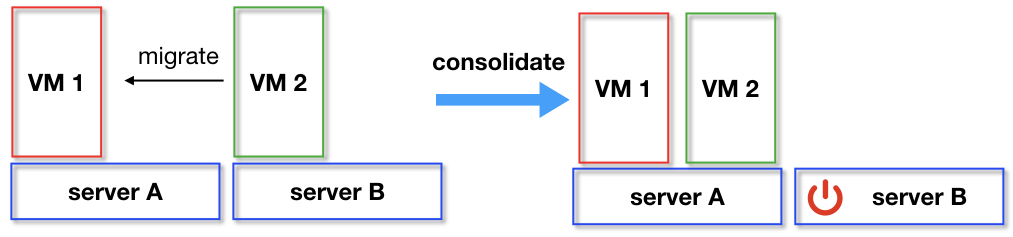
\includegraphics[width=0.7\textwidth]{pics/consolidate.png}
% 	\caption{A Server Consolidation example: Initially, each PM runs an application wrapped with a VM in a low resource utilization state. After the consolidation, both VMs are running on PM A, so that PM B is turned off to save energy \cite{Barroso:2007jt}.}
% 	\label{fig:consolidation}
% \end{figure}

% The low utilization of PM is also called \emph{Server Spawl} which means a large number of unnecessary PMs are running - result in large amount of extra energy consumption.
% The way of improving the resource utilization is through an effective resource allocation.

% Resource management in Cloud computing is a broad term including 
% various different strategies such as server 

% Server consolidation is achieved by manipulating the allocation of applications in the PMs so that the resource utilization of PMs achieve a high level. An effective resource allocation is affected by multiple factors such as virtualization technologies and distinct approaches in different scenarios or stages.

% Virtualization \cite{Uhlig:2005do} partitions a physical machine's resources (e.g. CPU, memory and disk) into several isolated units such as virtual machines (VMs) or containers. Traditional resource allocation is based on VMs, where Cloud providers offer a number fixed types of VM; Cloud users can select VMs by themselves - in Infrastructure as a Service (IaaS) or automatically select by a software platform provided by Cloud provider - in Platform as a Service (PaaS). 
\begin{figure}
	\centering
	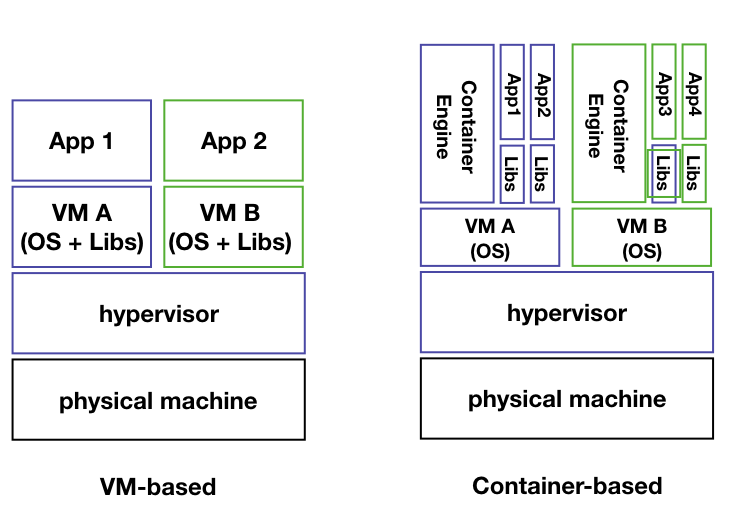
\includegraphics[width=0.7\textwidth]{pics/comparison.png}
	\caption{A comparison between VM-based and Container-based virtualization}
	\label{fig:comparison}
\end{figure}

Apart from these different resource allocation scenarios, we would also like to consider the server consolidation problem based on a new technology. Container technology \cite{Soltesz:2007cu} is an operating system level of virtualization. Each container wraps an application and multiple containers can be installed in a same operating system within a VM (see Figure \ref{fig:comparison} right-hand side). The reason for choosing container as the fundamental resource management unit is because
Container-based resource allocation can overcome three inherent disadvantages of VM-based resource allocation which cause low utilization in data centers.

\begin{itemize}
	% \item Resource management is based on VM. Cloud providers can dynamically adjust the location (in which PM) of a VM based on the observed resource utilization. 
	% \item Separated responsibilities of resource selection for applications and resource allocation. 
	% As above mentioned, Cloud users have to select the type of resources. This causes a problem. The accurate estimation is almost impossible because of unpredictable workloads; Cloud users tend to reserve more resources for ensuring the QoS at the peak hours \cite{Chaisiri:2012cv} than completely rely on auto-scaling, simply because auto-scaling is more expensive than reservation. However, the peak hours only account for a short period, therefore, in most of time, resources are wasted. As the types of VM are a part of the contract, Cloud providers cannot simply change the type of VMs after provisioning. 
	\item Resource over-provisioning \\
	As previous mentioned, VMs are either selected by Cloud users or automatically selected by software platforms. In either case, it requires an estimation of required resources. However, The accurate estimation is almost impossible because of unpredictable workloads; A simple way is to reserve more resources for ensuring the QoS at peak hours \cite{Chaisiri:2012cv}, rather than completely rely on auto-scaling, simply because auto-scaling is more expensive than reservation. However, the peak hours only account for a short period, therefore, in most of time, resources are wasted. In IaaS, the types of VM are a part of the contract, Cloud providers cannot simply change the type of VMs after provisioning. In PaaS, Cloud providers can change the type of VMs to more suitable sizes.

	% \item Cloud providers offer fixed types of VM. Because of the fixed size of resources and the one-on-one mapping of applications and VMs, specific applications consume unbalanced resources which leads to vast amount of resource wastage \cite{Tomas:2013iv}. For example, computation intensive tasks consume much more CPU than RAM; a fixed type of VM provides much more RAM than it needs. Because the tasks use too much CPU, they prevent other tasks from co-allocating. This also causes wastage. 
	\item Unbalanced usage of resources \\
	Specific applications consume unbalanced resources which leads to vast amount of resource wastage \cite{Tomas:2013iv}. For example, computation intensive tasks consume much more CPU than RAM; a fixed type of VM provides much more RAM than it needs. Because the tasks use too much CPU, they prevent other tasks from co-allocating. This also causes wastage.

	\item Heavy overhead of VM hypervisors and redundant operating systems (OSs) \\
	% Redundant operating systems (OSs) cause vast resource wastage. \\ 
	In VM-based resource allocation, heavy overhead is caused by
	the hypervisor of VMs and the separated operating systems running in the PM. A hypervisor manages and monitors the VMs running on a PM. The overhead of a hypervisor is heavier with the increasing numbers of VM. Redundant operating system is another reason for overhead, as normal applications do not need specific operating systems; Commonly used OSs - such as Linux-based: RedHat, or Windows server versions - are well enough for their needs. Therefore, running applications in separated operating system simultaneously is unnecessary.
\end{itemize}


Container-based allocation solves the over-provisioning problem by allocating multiple containers in the same VM. In addition, the unbalance resource problem can be solved by combining different types of applications (e.g CPU-intensive and Memory-intensive). Furthermore, because containers share a same VM, the overhead of hypervisor and OSs are naturally solved with less deployment of VMs.

% The recent development of container technology \cite{Soltesz:2007cu} is an operating system level of virtualization. Each container wraps an application and multiple containers can be installed in a same operating system within a VM (see Figure \ref{fig:comparison} right-hand side). Container technology has attracted the attention of both industrial and academia because it has the potential to solve these problems. 




% Apart from virtualization, different server consolidation strategies should be applied in different scenarios. This is because Cloud data center has a highly dynamic nature where it constantly receives new requests for resource allocation and releases of old resources, consequently, the energy efficiency is constantly dropping.





% In this thesis, our goal is to help Cloud providers to increase their profits by saving money from the energy consumed by servers.
% Specifically, we achieve this goal by providing better resource allocation techniques using the container-based server consolidation to optimize the resource utilization in different scenarios.

% The problem can be described as, a data center has a number of PMs, a number of types of VM and a number of containers to be allocated. They can be represented as resources 
% such as CPU cores and RAM. The task is to allocate these containers to a number of VMs, each of VM has a type. Furthermore, allocating these VMs to a minimum number of PMs. The decision variable is the location of containers and VMs as well as the types of VMs. The constraints are the aggregated resources of containers inside a VM cannot exceed the VM's capacity. Similarly, the aggregated resources of VMs inside a PM cannot exceed the PM's capacity. The main difficulty of the problem is a large number of combination container allocation and the choices of VMs which is too time-consuming for a brutal-force approach.

However, the new challenge posed by Container-based server consolidation is even harder than VM-based consolidation. Traditional VM-based server consolidation are modeled as bin-packing problems \cite{Mann:2015ua}. This is because VMs and PMs are naturally modeled as items and bins and server consolidation and bin-packing have the same optimization objective: minimize the number of bins/PMs. The complexity of bin-packing problem is NP-hard which means it is extreme time-consuming to find its optimal solution when the number of decision variables are large. In container-based server consolidation, there are two levels of allocation: Containers are allocated to VM as the first level and VMs are allocated to PMs as the second level. These two levels of allocation interact with each other, for the first level of allocation affects the decision in the second level. Therefore, it is necessary to propose new approaches for the problem.

Currently, most research focus on VM-based server consolidation and these methods can not be directly applied on container-based consolidation because of the different structure. Only few research focus on container-based server consolidation problem. One of the state-of-the-art research is from Piraghaj and et al \cite{Piraghaj:2015uf}. They first propose a VM-resizing technique that defines the types of VM based on analyzing the historical data from Google. Then they propose a two-step allocation: first allocate containers to VMs and then allocate VMs to PMs. Their major contribution is the method of defining types of VM. The allocation of containers does not optimize the energy consumption and the allocation of VMs are traditional First Fit algorithm. In addition, they propose a dynamic consolidation \cite{Piraghaj:2016bw} using a series simple heuristics such as Random Host Selection Algorithm or First Fit Host Selection. 
Their resource allocation system completely relies on dynamic consolidation without using static methods. Although their system can execute allocation fast, the energy efficiency cannot be guaranteed.
The reasons are mainly from two aspects, firstly, they mainly rely on simple bin-packing algorithms to allocate containers to VMs. As Mann's research \cite{Mann:2015ua} showed, server consolidation is a lot more harder than bin-packing problem because of the multi-dimensional of resources, many constraints. Therefore, general bin-packing algorithms do not perform well. Secondly, they use a two-step allocation. Because of the interaction of two allocations, separated optimization approach will lead to local optima \cite{Mann:2016hx}. Therefore, these two allocations should be considered simultaneously.

% Deterministic methods such as Integer Linear Programming \cite{Speitkamp:2010ck} and Mixed Integer Programming \cite{Wang:2016eh} have been used but they are well-known that they are very time-consuming for a large scale problem. 
% More research proposed heuristic methods to approximate the optimal solution such as 
% First Fit Decreasing (FFD) \cite{Panigrahy:2011wk}, Best Fit Decreasing (BFD) \cite{Beloglazov:2012ji}.
% Manually designed heuristics are designed to tackle the special requirements such 
% as a bin-item incomplete scenario \cite{Gupta:2008ul} and multi-tier applications \cite{Jung:2008vb, Li:2009wf}. Although these greedy-based heuristics can quickly approximate an answer,  as Mann's research \cite{Mann:2015ua} showed, server consolidation is a lot more harder than bin-packing problem because of the multi-dimensional, many constraints. Therefore, general bin-packing algorithms do not perform well with many constraints and specific designed heuristics only perform well in very narrow scope.

% Although traditional VM-based server consolidation has been studied for year, these methods can not be directly applied on container-based problem because container-based consolidation has two levels of allocation: Containers are allocated to VM as the first level and VMs are allocated to PMs as the second level. These two levels of allocation interact with each other, for the first level of allocation affects the decision in the second level.



% The most important feature of container is that it utilizes the resources inside VMs. 
% Therefore, even CaaS is also built upon IaaS, it solves the fixed types by allocating containers in it. This feature also solves the redundant operating systems problem.
% The second characteristic is that a container's size is changeable and can be controlled by 
% Cloud provider in real-time. Therefore, the Cloud providers can monitor the resource utilization of applications and adjust it accordingly. This feature provides better flexibility which solves the over-provisioning problem. 
% In addition, one feature that separates CaaS and PaaS is that, containers allow user-defined libraries instead of constrained by the platform.


% The way of improving the resource utiltization is called server consolidation.



% Server consolidation can be applied on different virtualization technologies and at different resource management stages in data center. 


% Therefore, Cloud providers objective is to maximize utilization of computing resources. A high utilization brings two benefits, firstly, it increases income by accommodating more applications in limited resources. Secondly, it cuts the expense of energy consumption by packing applications in a minimum number of PMs so that idle PMs can be turned off. 	




% \begin{figure}
% 	\centering
% 	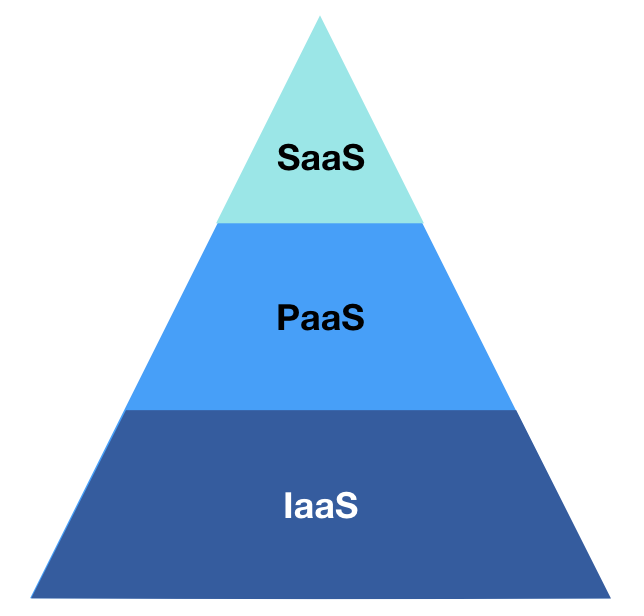
\includegraphics[width=0.5\textwidth]{pics/pyramid.png}
% 	\caption{Pyramid of service models in Cloud computing. 
% 	IaaS provides the fundamental resources such as CPU cores, RAM. The resources are usually wrapped with various types of virtual machine. PaaS provides a software platform sitting on top of IaaS for Cloud users to develop applications. SaaS is the application that serves End Users.}
% 	\label{fig:pyramid}
% \end{figure} 


% Service models of Cloud computing are critical in solving energy consumption problem because their distinct ways of managing resources have sever effect on the problem. These distinct ways of resource management mainly result from the responsibilities among stakeholders. There are three traditional service models \cite{Mell:2011jj}: Infrastructure as a Service (IaaS), Platform as a Service (PaaS) and Software as a Service (SaaS). The relationship among three service models can be pictured as a pyramid (see \ref{fig:pyramid}). Their detailed responsibilities among stakeholders are explained as below:


% \begin{itemize}
% 	\item IaaS, a Cloud provider hosts hardwares such as PMs and cooling infrastructure on behalf of Cloud users. A Cloud provider also provides maintenance, management of hardware resources. 

% 	In IaaS, Cloud provider offers the fundamental resources such as CPU cores, RAMs, and network bandwidth. These resources are often encapsulated in virtualized computing units called virtual machines (VMs). Cloud providers establish a number of types of VM for simplifying the management. The `type' means a VM contains a certain quantity of resources such as 2-cores and 1 GB RAM.  \emph{Traditional} IaaS and PaaS use VM as the fundamental unit of resources.

% 	A typical procedure of a Cloud user deploying their applications in an IaaS cloud includes several steps.
% 	Initially, Cloud users estimate the resources that their applications might consume and select a type of VM which can satisfy the requirement. After Cloud users have made the decisions, they send requests to Cloud providers for a number of VMs. Finally, Cloud providers received the request, provisioned and allocated these VMs to PMs. 

% 	From the resource management perspective, the constraint in allocation of VMs is that the aggregated VMs' resources in a PM cannot exceed the capacity of the PM. After these VMs have been allocated, their types cannot be changed. During the life cycle of an application, Cloud providers can dynamically adjust the locations of VMs, provision new VMs (same type) for the replicas of an application, as well as turning on/off PMs.

	% After receiving the requests, Cloud providers choose a set of PMs which contains sufficient resources, provision the required VMs in them. Then, the VMs are assigned to the Cloud users. Cloud providers manage the VMs by monitoring the resource utilization of VMs and PMs. If a VM has run out of resources, an auto-scaling strategy is used to provision new VMs to Cloud users. Finally, Cloud providers optimize the locations of VMs so that the energy consumption of data center is minimized.


 	% \item PaaS, a Cloud provider offers a platform which allows Cloud users to develop, test and deploy their applications on it.

 	% From resource management perspective, as shown in Figure \ref{fig:pyramid}, PaaS is sitting above the IaaS which means the underlying resource is still based on IaaS VM types. Different from IaaS, PaaS takes the responsibility of selecting VMs and allows Cloud users to focus on software development. 

 	% A typical procedure of a Cloud user deploying their applications in an PaaS cloud includes several steps.
 	% In the first step, Cloud users need to provide the initial estimation of the quantity of resources instead of types of VM. Then, Cloud providers determine the types of VM for applications according to the estimated resources.  After this step, resource management system conducts the provisioning and allocating as the same steps in IaaS. During the life cycle of applications, similar to IaaS, Cloud providers can also adjust the location of VMs, add new VMs, and control the status of PMs. Different from IaaS, Cloud providers can change the type of VM for an application as long as the application's performance can be guaranteed.

 	% The system monitors the utilization of a number of PM and VM and through adjustment of their location to optimize the energy consumption of the data center. The input is a list of VMs (e.g CPU cores and RAMs) and a list of PMs. The task is to put the VMs into these PMs so that the VMs only use a minimum number of PMs. The sizes of VMs and PMs are fixed. A system can only adjust which VM is allocated to which PM. A general constraint is the sum of resources of the VMs inside a PM cannot exceed the capacity of the PM.

%  	\item SaaS describes the relationship between Cloud users and End users. End users create workloads for applications. Although this service model does not directly related to the resource management, it provides the fundamental reasons for resource management and optimization. Because of the dynamic nature of workloads, the underlying resources must also be dynamic adjusted to meet the requirement.
% \end{itemize}

% In this proposal, we focus on an important issue of helping Cloud providers to improve their profit. Our approach is to reduce the expense of energy consumption in data centers by providing a series of optimization methods in Cloud data center resource management. The centric idea of resource management is to decide the location a set of applications in a minimum number of physical machines 
% so that the energy consumption of PMs are minimized. 

% Our proposed optimization approaches are based on a new service model: Container as a Service (CaaS) \cite{Piraghaj:2016bw} which is a variant of PaaS. The reasons for us to establish our approaches on CaaS are listed as followed:
% \begin{itemize}
% 	\item CaaS uses a new virtualization technology called containers which has shown several important characteristics that overcome the disadvantages of traditional IaaS and PaaS, therefore, CaaS is a promising trend.
% 	\item CaaS has a fine granularity level of resource management which has shown opportunities to improve the resource utilization, however, it often proposes new optimization challenges which have not been studied yet.
% \end{itemize}

% % Before explaining the details of resource management strategies, we first illustrate several characteristics of resource management in IaaS.
% Firstly, we illustrate the disadvantages of traditional IaaS and PaaS and discuss the reasons of why current approaches cannot completely overcome these problems. From there, we explain why CaaS is a prescription of their problems.

% IaaS has three characteristics which naturally lead to a low resource utilization.
% \begin{itemize}
% 	% \item Resource management is based on VM. Cloud providers can dynamically adjust the location (in which PM) of a VM based on the observed resource utilization. 
% 	\item Separated responsibilities of resource selection for applications and resource allocation. 
% 	As above mentioned, Cloud users have to select the type of resources. This causes a problem. The accurate estimation is almost impossible because of unpredictable workloads; Cloud users tend to reserve more resources for ensuring the QoS at the peak hours \cite{Chaisiri:2012cv} than completely rely on auto-scaling, simply because auto-scaling is more expensive than reservation. However, the peak hours only account for a short period, therefore, in most of time, resources are wasted. As the types of VM are a part of the contract, Cloud providers cannot simply change the type of VMs after provisioning. 

% 	\item Cloud providers offer fixed types of VM. Because of the fixed size of resources and the one-on-one mapping of applications and VMs, specific applications consume unbalanced resources which leads to vast amount of resource wastage \cite{Tomas:2013iv}. For example, computation intensive tasks consume much more CPU than RAM; a fixed type of VM provides much more RAM than it needs. Because the tasks use too much CPU, they prevent other tasks from co-allocating. This also causes wastage. 

% 	\item Redundant operating systems (OSs) cause vast resource wastage. Since each VM runs a separated operating system, a PM might run many operating systems at a time. However, normal applications do not need specific operating systems commonly used OSs - such as Linux-based: RedHat, or Windows server versions - are well enough for their needs. Therefore, running duplicated OSs in a PM is unnecessary.
% \end{itemize}

% For the first two drawbacks, previous researchers and developers have come up with two strategies: server consolidation and overbooking.

 

% \emph{Server consolidation} \cite{Zhang:2010vo}, as above mentioned, utilized a dynamic migration technique to resolve the low utilization problem by gathering applications into a fewer number of PMs (see Figure \ref{fig:consolidation}), so that the resource utilization of PMs are maintained at a high level. In the meanwhile, idle PMs can be turned off to save energy. Consolidation dramatically improves hardware utilization and lowers PM and cooling energy consumption. 

% \emph{Overbooking} strategy \cite{Tomas:2013iv} is used to overcome the low utilization problem raised by the over-provisioning\cite{Chaisiri:2012cv} of VMs. Over-provisioning means Cloud users choose more resources than their needs. It allocates more VMs in a PM even their aggregated resources have exceeded the PM's capacity. The advantage of this approach is that, indeed, it improves the resource utilization. The disadvantages are also obvious: if one or more applications are experiencing a heavy load; the PM is likely to run out of resources. At this moment, all the applications are suffer from a QoS degradation. In order to avoid the overloading, Cloud users often carefully predict the utilization of applications based on their previous workloads, when applications start degrading, a dynamic resource management approach is used to adjust the VMs' location.

% \begin{figure}
% 	\centering
% 	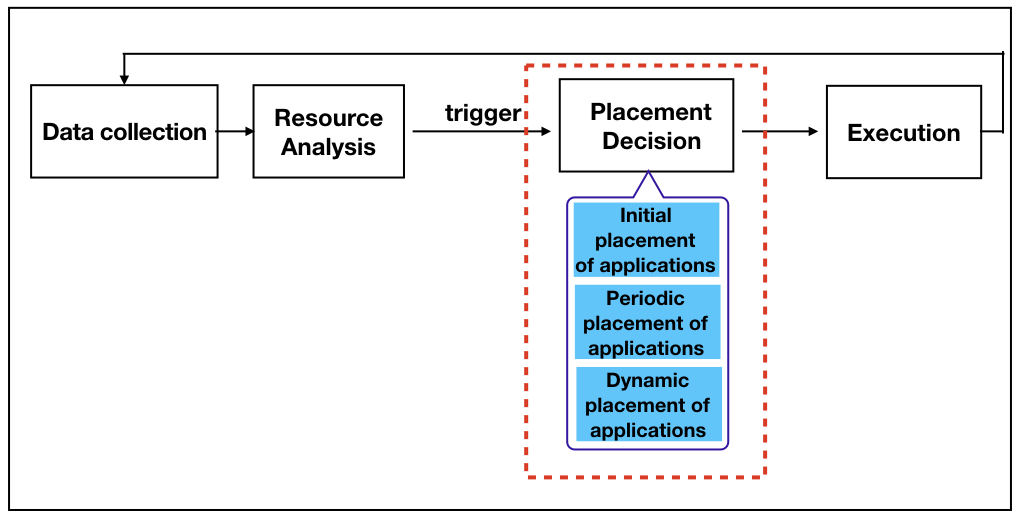
\includegraphics[width=0.7\textwidth]{pics/workflow_management.png}
% 	\caption{A workflow of resource management \cite{Mishra:2012kx}}
% 	\label{fig:workflow}
% \end{figure}

% The work-flow of utilizing these two strategies in resource management is shown in Figure \ref{fig:workflow}. 
% It seemingly solves the over-provisioning problem, however, the overbooking strategy brings new challenges. Although the overbooking strategy have been studies for years \cite{}, the prediction of workload is very difficult \cite{} or even impossible as referred in many literatures \cite{}. The improvement of resource utilization is completely based on an accurate prediction of a large number of applications. Its effectiveness is hard to evaluate and justify. It is also very time consuming to predict the utilization of every application. Therefore, it is urgent to provide a strategy without making a prediction. One possible way is to use finer granularity strategy of resource management.

% Furthermore, there is no solution for the third drawback in the context of IaaS.

% For traditional PaaS, Cloud providers can adjust the applications' location and the type of VM. Therefore, it overcomes the first drawback of IaaS. Because of PaaS is built upon IaaS, the one-on-one relationship between application and VM still exist. PaaS can only select the most suitable type instead of changing their sizes. Therefore, the unbalanced resource problem cannot be solved. In addition, PaaS brings a restriction for the applications deployed on it. PaaS build a software middle-ware to allow Cloud users' development. The middle-ware requires the deployed applications to be compatible with the environment, for example, Google App engine \cite{} only allows certain programming languages and libraries. Therefore, the generality of PaaS is limited. It is urgent to provide a environment which supports automatic resource management as well as an editable programming environment.

% The recent development of container technology \cite{Soltesz:2007cu} has driven the attention of both industrial and academia because its potential to solve these problems in both IaaS and PaaS.
% Container is an operating system level of virtualization which means multiple containers can be installed in a same operating system (see Figure \ref{fig:comparison} right-hand side). Each container provides an isolated environment for an application. In short, a VM is partitioned into smaller manageable units. 
% Container as a Service (CaaS) is a variant of PaaS propose by a leading Lab in this field \cite{Piraghaj:2015uf}. 
% Instead of VMs, CaaS uses both container and VM as a hybrid resource management unit.

% \begin{figure}
% 	\centering
% 	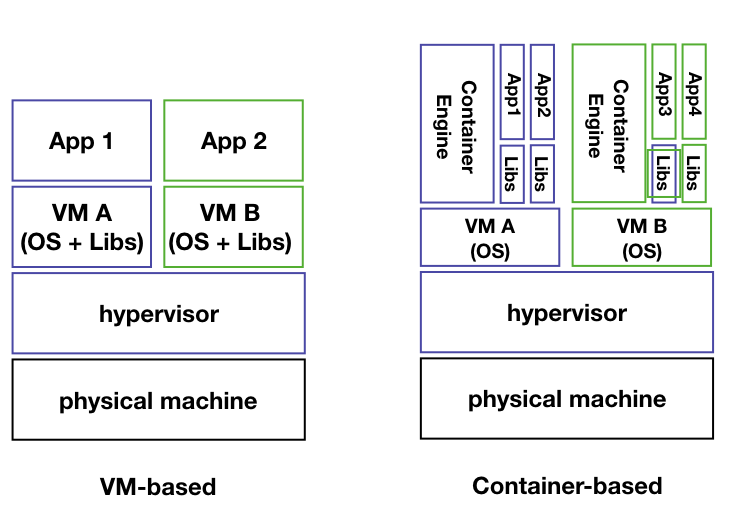
\includegraphics[width=0.7\textwidth]{pics/comparison.png}
% 	\caption{A comparison between VM-based and Container-based virtualization}
% 	\label{fig:comparison}
% \end{figure}

% CaaS solves the problems in IaaS and PaaS because of containers' characteristics.
% The most important feature of container is that it utilizes the resources inside VMs. 
% Therefore, even CaaS is also built upon IaaS, it solves the fixed types by allocating containers in it. This feature also solves the redundant operating systems problem.
% The second characteristic is that a container's size is changeable and can be controlled by 
% Cloud provider in real-time. Therefore, the Cloud providers can monitor the resource utilization of applications and adjust it accordingly. This feature provides better flexibility which solves the over-provisioning problem. 
% In addition, one feature that separates CaaS and PaaS is that, containers allow user-defined libraries instead of constrained by the platform.

% Although CaaS has these promising characteristics, it also proposes a difficult research problem. In order to 
% understand the difficulty of the problem, it is necessary to illustrate the difficulty of current VM-based server consolidation problem.


% Currently, vast amount of server consolidation methods are mostly VM-based and they are mainly modeled as bin-packing problems \cite{Mann:2015ua}. This is because VMs and PMs are naturally modeled as items and bins and server consolidation and bin-packing have the same optimization objective: minimize the number of bins/PMs. The complexity of bin-packing problem is NP-hard which means it is extreme time-consuming to find its optimal solution when the number of decision variables are large. Deterministic methods such as Integer Linear Programming \cite{Speitkamp:2010ck} and Mixed
% Integer Programming \cite{Wang:2016eh} have been used but they are well-known that they are very time-consuming for a large scale problem. 
% More research proposed heuristic methods to approximate the optimal solution such as 
% First Fit Decreasing (FFD) \cite{Panigrahy:2011wk}, Best Fit Decreasing (BFD) \cite{Beloglazov:2012ji}.
% Manually designed heuristics are designed to tackle the special requirements such 
% as a bin-item incomplete scenario \cite{Gupta:2008ul} and multi-tier applications \cite{Jung:2008vb, Li:2009wf}. Although these greedy-based heuristics can quickly approximate an answer,  as Mann's research \cite{Mann:2015ua} showed, server consolidation is a lot more harder than bin-packing problem because of the multi-dimensional, many constraints. Therefore, general bin-packing algorithms do not perform well with many constraints and specific designed heuristics only perform well in very narrow scope.

% Although traditional VM-based server consolidation has been studied for year, these methods can not be directly applied on container-based problem because container-based consolidation has two levels of allocation: Containers are allocated to VM as the first level and VMs are allocated to PMs as the second level. These two levels of allocation interact with each other, for the first level of allocation affects the decision in the second level.

% As a variant of PaaS, it allows Cloud providers to manage both the resource selection and resource allocation. Specifically,  
% When an application is initially deployed, the Cloud user need to provide an initial estimation of resources. Cloud provider wraps the application with a container according to the estimated size and allocates it to a PM. During the life cycle of the application, the size of the container can be adjusted according to its resource utilization. Like VMs, containers can also be migrated among VMs. These flexibility allows Cloud providers to utilize the resources in VM more efficiently, hence, solved the fixed types of VM problem. 

% Containers also solve the problem of limited software development environment by providing user-defined libraries. Each application 
% can have distinct libraries but share the kernel of a same operating system. This surely solve the redundant operating system problem since large amount of application only needs the basic functionalities of an operating system such as memory management.


% Hence, Cloud providers have a complete control of resources which may result in a better utilization of resources. 
% In addition, IaaS Cloud runs many redundant operating systems and hypervisors. CaaS eliminates these redundancies by a single operating system with multiple containers.

% \begin{figure}[H]
% 	\centering
% 	\begin{subfigure}[b]{0.45\textwidth}
% 		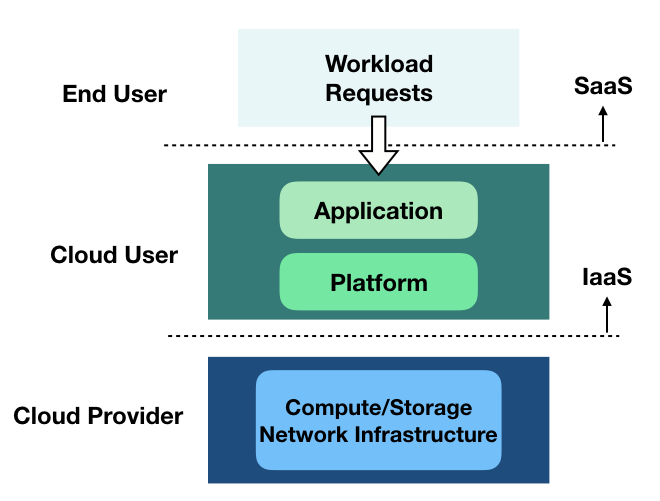
\includegraphics[width=\textwidth]{pics/iaas.png}
% 		\caption{IaaS + SaaS}
% 	\end{subfigure}
% 	\begin{subfigure}[b]{0.45\textwidth}
% 		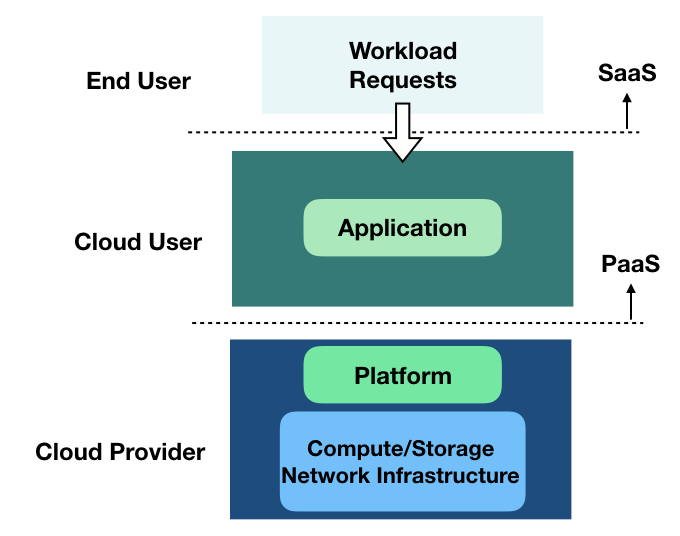
\includegraphics[width=\textwidth]{pics/paas.png}
% 	\caption{PaaS + SaaS}
% 	\end{subfigure}
% 	\caption{Three Service models \cite{Jennings:2015ht}}
% 	\label{fig:service_models}
% \end{figure}

% \begin{itemize}
%  	\item \emph{IaaS}, Cloud provider offers the fundamental computing resources, often in a form of various sizes of VMs. Apart from the virtualized hardware and operating systems, Cloud users treat the remote VMs as local; they can build a project-specific platform on it and deploy their applications. In terms of resource management, Cloud users have the responsibility to estimate the quantity of resources, while Cloud providers have no knowledge or control of what inside VMs. Resource management is based on VM. 
  	
%   	\item \emph{PaaS}, Cloud providers establish the software development platform to enable the in-progress software to be developed in the platform.  The main difference between PaaS and IaaS is that, in PaaS, Cloud providers not only offer the hardwares but also a platform which allows software development. In terms of resource management, Cloud providers have the full control of resource allocation. Therefore, Cloud users can focus on software development.
  	
%   	\item \emph{SaaS} describes application built and maintain by Cloud users; applications are then available for the End users via the Internet. Many SaaS products are built by companies who use IaaS or PaaS. Therefore, it does not involve with resource management. 
% \end{itemize}



% The solution of the high energy consumption problem comes two important aspects: Virtualization technology which enables a fine granularity resource management and various strategies which are tight coupling with service models. 





% 

% With virtualization, IaaS and PaaS applied different strategies in resource management.
% In PaaS, Cloud providers are responsible for the application 
% In IaaS, Cloud providers offer Cloud users a set of types of VM. The term ``type'' here means different types of VM contains distinct quantity of resources such as CPU cores, memory, and network bandwidth. A Cloud user must estimate the resource consumption of their applications and choose an appropriate type of VM.
% This step is addressed as resource mapping \cite{}. Cloud providers receive the VM provisioning requests and start to manage resources. 


%  The first characteristic inspires a strategy called \emph{server consolidation}; the second and third inspire an \emph{overbooking} strategy. These two strategies are collaborated to achieve a better utilization. For last characteristics, so far, it lacks effective ways to solve them.



% This new concept starts a new service model called Container as a Service (CaaS) . CaaS brings advantages for both Cloud customers and providers.
% From Cloud users' perspective, CaaS has advantages of both IaaS (Infrastructure as a Service) and PaaS (Platform as a Service) but without their disadvantages. On one hand - similar to PaaS - it does not require Cloud users to estimate the quantity of resources so that they can focus on application development. On the other hand - similar to IaaS - it allows Cloud users to customize their software environment without being constrained by platforms. 

% For Cloud provides, CaaS resolves two IaaS's inherent weaknesses which cause low utilization of resources.



% In contrast, CaaS solves above two problems at a time. 

% \vspace{10mm}




% Evolutionary Computation (EC) is commonly used to solve combinatorial optimization problem \cite{Guzek:2015ds}, therefore, it is particular useful in solving the global consolidation problem.  Many EC techniques including Genetic Algorithm (GA) \cite{Xu:2010vh}, Ant Colony Optimization (ACO) \cite{Gao:2013gg, Mateos:2013bm}, Particle Swarm Optimization (PSO) \cite{Jeyarani:2012fg} have been used in solving this problem. EC algorithms show their advantages in the following aspects. Firstly, EC algorithms are good at solving multi-objective problems because of their population-based nature. And global consolidation problem often involves two or more objectives (e.g energy efficiency and migration cost). Secondly,  they can provide near-optimal solutions within a reasonable amount of time.  

% In VM-based dynamic problem, 
% previous most research proposed human designed greedy-based dispatching rules or heuristics such as a First-Fit-based approach \cite{Bobroff:2007ec}, Modified Best Fit Decreasing \cite{Beloglazov:2012ji}, and a two-stage heuristic \cite{Zhang:2015jm}. One of the major problem for human designed heuristics is that if any inherent component gets changes, then the designed heuristic may not work as it was expected \cite{SoteloFigueroa:2013be}. EC algorithms are also seldom considered in this scenario because most EC methods need more time to search through solutions space.

%  As Mann illustrated in \cite{Mann:2016hx},  these two steps should be conducted simultaneously, otherwise it leads to local optimal. Other research \cite{Dong:2014iz, Hindman:2011ux, Anselmi:2008ik} propose greedy-based heuristics on container allocation problem. They can be easily stuck at local optimal. 
% This thesis, therefore, aims at providing an end-to-end solution for Container-based server consolidation which includes three stages correspond with the Cloud resource management procedure (see Figure \ref{fig:management}): initialization, static container-based server consolidation and dynamic container placement.

% Despite the usefulness of server consolidation, it is a difficult task. Traditional server consolidation is conducted manually \cite{Chebiyyam:2009uq} with vast data analysis and interviews with application owners. It is fraught and extremely difficult to reach a global optima state.
% Later on, server consolidation is often considered as a global optimization problem 
% where its goal is to minimize the overall energy consumption. 
% It is often modeled as a bin-packing problem \cite{Mann:2015ua} which is a well-known NP-hard problem meaning it is unlikely to find an optimal solution of a large problem. 

% In static methods, deterministic methods such as  
% Integer Linear Programming \cite{Speitkamp:2010ck} and Mixed
% Integer Programming \cite{Wang:2016eh} are often considered. However, it is well-known that they are very time-consuming for a large scale problem. More research proposed heuristic methods
%  to approximate the optimal solution such as 
% First Fit Decreasing (FFD) \cite{Panigrahy:2011wk}, Best Fit Decreasing (BFD) \cite{Beloglazov:2012ji}.
% Manually designed heuristics are designed to tackle the special requirements such 
% as a bin-item incomplete scenario \cite{Gupta:2008ul} and Multi-tier Applications \cite{Jung:2008vb, Li:2009wf}. Although these greedy-based heuristics can quickly solve the consolidation problem,  as Mann's research \cite{Mann:2015ua} shown, server consolidation is a lot more harder than bin-packing problem because of multi-dimension, many constraints. Therefore, a simple greedy-based heuristic (e.g FFD) leads to a bad performance. 

% Evolutionary Computation (EC) is commonly used to solve combinatorial optimization problem \cite{Guzek:2015ds}, therefore, it is particular useful in solving the global consolidation problem.  Many EC techniques including Genetic Algorithm (GA) \cite{Xu:2010vh}, Ant Colony Optimization (ACO) \cite{Gao:2013gg, Mateos:2013bm}, Particle Swarm Optimization (PSO) \cite{Jeyarani:2012fg} have been used in solving this problem. EC algorithms show their advantages in the following aspects. Firstly, EC algorithms are good at solving multi-objective problems because of their population-based nature. And global consolidation problem often involves two or more objectives (e.g energy efficiency and migration cost). Secondly,  they can provide near-optimal solutions within a reasonable amount of time.  

% Dynamic consolidation problem requires fast decision-making and global optimization. Previous most research proposed human designed greedy-based dispatching rules or heuristics such as a First-Fit-based approach \cite{Bobroff:2007ec}, Modified Best Fit Decreasing \cite{Beloglazov:2012ji}, and a two-stage heuristic \cite{Zhang:2015jm}. One of the major problem for human designed heuristics is that if any inherent component gets changes, then the designed heuristic may not work as it was expected \cite{SoteloFigueroa:2013be}. EC algorithms are also seldom considered in this scenario because most EC methods need more time to search through solutions space.

